\documentclass[twocolumn]{article}
\usepackage[spanish]{babel}
\usepackage{caption}
\usepackage{graphicx}
\usepackage{amsmath}
\setlength{\parindent}{0pt}

\author{Josué Villasante}
\title{Interferómetro}

\begin{document}
	\maketitle

	\section{Objetivo}
		Crear un patrón de interferencia producido por la división y posterior unión de un mismo haz de luz de un láser.

	\section{Procedimiento}
		El láser utilizado tuvo una potencia menor a 20mW y una longitud de onda de 633nm.

		Primero se empezó alineando el haz de luz luego de los dos primeros espejos, para que este esté siga la línea de orificios en la mesa. Luego se colocó la lamina retardadora y el PBS (polarizing beam splitter) lo más cercano al segundo espejo, y se intentó alinear el haz del láser polarizado verticalmente de manera paralela a los orificios de la mesa. Rápidamente, se observó que no se podía alinear este haz sin evitar que parte del reflejo del PBS regrese al láser produciendo un haz distorsionado.

		\begin{center}
			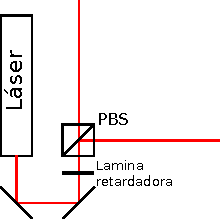
\includegraphics[width=100pt]{img/layout_attempt.pdf}
			\captionof{figure}{Arreglo de primera configuración.}
		\end{center}

		Por lo tanto, para evitar la distorsión se colocó la lamina retardadora y el PBS a una mayor distancia del segundo espejo, y, por otro lado, se colocó un iris inmediatamente luego del láser. La mayor distancia permitió que el desvío de la reflexión sea mayor. El iris se utilizó para bloquear este haz de luz reflejado por el PBS.

		Se continuó colocando el espejo 3 y 4, e igualmente se alineó ambos hazes con los orificios de la mesa. Luego se colocó el BS (beam splitter) y se lo alineó de tal forma que produzca un solo punto en ambos lados. Hasta ese momento no se observó ningún patrón de interferencia.

		\begin{center}
			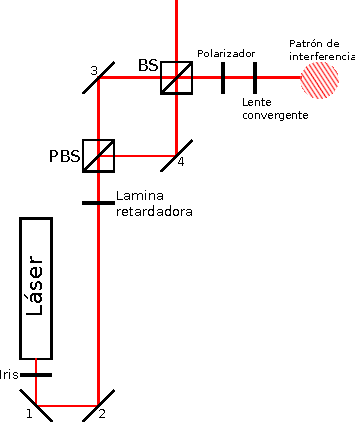
\includegraphics[width=150pt]{img/layout.pdf}
			\captionof{figure}{Arreglo final del experimento.}
			\label{final_layout}
		\end{center}

		Para observar el patrón era necesario colocar un polarizador a 45$^{\circ}$. Para esto se colocó temporalmente el polarizador entre el espejo 3 y el PBS, y se lo rotó hasta encontrar la posición con menor potencia (sin mover el indicador de ángulo). La menor potencia encontrada fue alrededor de 5$\mu W$. Posteriormente, usando las marcas de ángulos del polarizador, se lo rotó hasta marcar 45$^{\circ}$. Con el polarizador listo, se lo movió a su posición final en la mesa tal cómo se ve en la figura \ref{final_layout}.

		A partir de este momento se ya pudo observar el patrón de interferencia en cualquiera de los puntos resultantes. Para agrandar el punto resultante se colocó un lente convergente, y se pudo ver claramente el patrón.

	\section{Resultados}
		El patrón de interferencia observado fue el siguiente.

		\begin{center}
			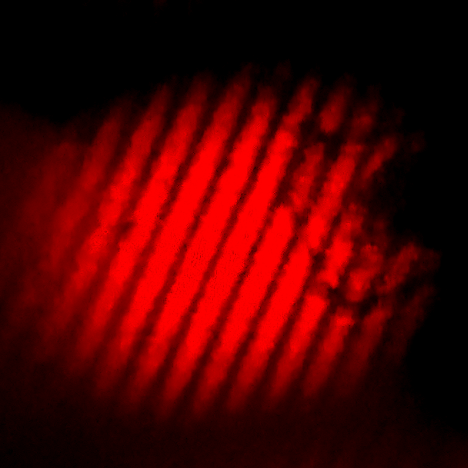
\includegraphics[width=100pt]{img/interference.png}
			\captionof{figure}{Patrón de interferencia observado.}
			\label{interference}
		\end{center}
\end{document}